\section{Analisi del dominio}

% 2.1.1
\subsection{Caratteristiche}
Ogni agente presente nella simulazione è stato modellato sulla base delle caratteristiche presenti nel modello IMPACT \cite{vanderWal2017Model}, quindi è contraddistinto da:

\begin{itemize}
 \item \textbf{Età}: bambino, adulto o anziano.
 \item \textbf{Sesso}: uomo, donna.
\end{itemize}

L'appartenenza ad uno dei gruppi sociali costituiti dalla combinazione di queste due proprietà determina:

\begin{itemize}
 \item \textbf{Velocità}: basata sulle osservazioni presenti in \cite{Willis2004} e distinta tra camminata e corsa da un fattore moltiplicativo.
 \item \textbf{Conformità alle regole}: valore tra 0 e 1 fisso per ogni gruppo sociale e stabilito a partire dai dati raccolti in \cite{Soto2011}.
 \item \textbf{Attitudine ad aiutare}: probabilità che un agente vada in soccorso di un altro considerando, il gruppo sociale di appartenenza di entrambi ed il loro legame.
\end{itemize}

\begin{table}[ht]
\centering
\renewcommand{\arraystretch}{1.5}
\begin{tabular}{|c|c|c|}
\hline
\textbf{Peso}       & \textbf{Descrizione}                                  & \textbf{Valore}   \\ \hline
$\omega_{s}$        & Capacità di percepire il pericolo                     & 0.5               \\ \hline
$\omega_{ab}$       & Influenza della paura sulla sensazione di pericolo    & 1.0               \\ \hline
$\omega_{p}$        & Persistenza dell'emozione                             & 0.95              \\ \hline
$\omega_{af}$       & Amplifica la paura                                    & 1.0               \\ \hline
$\omega_{if}$       & Inibisce la paura                                     & -0.5              \\ \hline
$\omega_{ae}$       & Amplifica il desiderio di evacuare                    & 1.0               \\ \hline
$\omega_{iw}$       & Inibisce il desiderio di evacuare                     & -1.0              \\ \hline
$\omega_{ai}$       & Amplifica l'intenzione di evacuare                    & 1.0               \\ \hline
$\omega_{ii}$       & Inibisce l'intenzione di evacuare                     & -1.0              \\ \hline
\end{tabular}
\caption{Tabella dei pesi utilizzati nel modello IMPACT.}
\label{table:weights-impact}
\end{table}

\begin{table}[ht]
\centering
\renewcommand{\arraystretch}{1.5}
\begin{tabular}{|c|c|c|}
\hline
\textbf{Simbolo}                                & \textbf{Formula}                                                  \\ \hline
$E(d(t))$                                       & $\frac{\sum_{i=1}^{n} d_{i}(t)}{n}$                               \\ \hline
$E(f(t))$                                       & $\frac{\sum_{i=1}^{n} f_{i}(t)}{n}$                               \\ \hline
$sig_{\sigma \tau}(V_{1}, ..., V_{k})$          & $\frac{1}{1 + e^{-\sigma(V_{1} + ... + V_{k} - \tau)}}$           \\ \hline
$asig_{\sigma \tau}(V_{1}, ..., V_{k})$         & $(\frac{1}{1 + e^{-\sigma(V_{1} + ... + V_{k} - \tau)}} - \frac{1}{1 + e^{\sigma \tau}})(1 + e^{-\sigma \tau})$ \\ \hline
\end{tabular}
\caption{Tabella delle formule utilizzate nelle equazioni del modello IMPACT.}
\label{table:formulas-impact}
\end{table}

Vi sono inoltre delle caratteristiche che evolvono durante la simulazione seguendo i principi del Network Oriented Modeling. Le equazioni relative ad ognuna di esse sono state decontestualizzate rispetto allo specifico scenario proposto nel modello IMPACT, per permetterne un utilizzo più generico anche all'interno di altre ambientazioni. \newline 
Per una esaustiva comprensione del funzionamento di queste proprietà, è utile consultare la tabella \ref{table:weights-impact}, dove sono descritti i pesi $\omega$ impiegati e la tabella \ref{table:formulas-impact}, in cui sono riassunti i simboli e le relative formule che sono state inserite nelle equazioni per favorirne la leggibilità. \newline
Nell'interpretare il significato delle varie caratteristiche è doveroso specificare la differenza tra il concetto di desiderio e quello di intenzione; per farlo ci si può affidare ad un esempio: un pedone bloccato a terra in seguito ad una caduta, ha mentalmente un forte desiderio di fuggire, ma non riuscendoci fisicamente ha al contempo una bassa intenzione di andarsene.

\begin{itemize}
    \item \textbf{Sensazione di pericolo ($d(t)$)}: influenzata dalla vicinanza al pericolo in un qualsiasi momento $pos(t)$, dal livello di paura dell'agente $f(t)$ e, per contagio sociale, dal livello di pericolo medio percepito dagli altri agenti $E(d(t))$.
    \begin{equation*}
        d(t + \Delta t) = d(t) + \eta(max(\omega_{s} \cdot pos(t), \omega_{p} \cdot d(t), \frac{\omega_{ab} \cdot f(t) + E(d(t))}{\omega_{ab} + 1}) - d(t))\Delta t
    \end{equation*}
    
    \item \textbf{Paura ($f(t)$)}: ottenuto dal desiderio di fuggire $e_{d}(t)$, quello di non fuggire $r_{d}(t)$ e dal livello di paura degli agenti nella simulazione $E(f(t))$.
    \begin{equation*}
        f(t + \Delta t) = f(t) + \eta(max(\omega_{p} \cdot f(t), asig(E(f(t)), w_{af} \cdot e_{d}(t), w_{if} \cdot r_{d}(t))) - f(t))\Delta t
    \end{equation*}
    
    \item \textbf{Desiderio di fuggire ($e_{d}(t)$)}: calcolato considerando la conformità alle regole $\chi$ del pedone, il livello di paura attuale $f(t)$ e la sensazione di pericolo $d(t)$.
    \begin{equation*}
        e_{d}(t + \Delta t) = e_{d}(t) + \eta(\chi \cdot max(\omega_{ae} \cdot d(t), \omega_{ae} \cdot f(t)) - e_{d}(t))\Delta t
    \end{equation*}
 
    \item \textbf{Desiderio di non fuggire ($r_{d}(t)$)}: sentimento contrapposto al precedente ottenuto combinando gli stessi parametri con differenti pesi.
    \begin{equation*}
        r_{d}(t + \Delta t) = r_{d}(t) + \eta(\chi \cdot (1 - max(\omega_{iw} \cdot d(t), \omega_{iw} \cdot f(t))) - r_{d}(t))\Delta t
    \end{equation*}

    \item \textbf{Intenzione di fuggire ($e_{i}(t)$)}: stabilisce il livello di convinzione a fuggire del pedone a partire dai valori delle due caratteristiche precedenti. 
    \begin{equation*}
        e_{i}(t + \Delta t) = e_{i}(t) + \eta(e_{d}(t) \cdot sig(\omega_{ai} \cdot e_{d}(t), \omega_{ii} \cdot r_{d}(t)) - e_{i}(t))\Delta t
    \end{equation*}
    
    \item \textbf{Intenzione di non fuggire ($r_{i}(t)$)}: confrontato con l'intenzione di fuggire $e_{i}(t)$ per determinare la scelta del pedone.
    \begin{equation*}
        r_{i}(t + \Delta t) = r_{i}(t) + \eta(e_{d}(t) \cdot sig(\omega_{ii} \cdot e_{d}(t), \omega_{ai} \cdot r_{d}(t)) - r_{i}(t))\Delta t
    \end{equation*}
\end{itemize}

% 2.1.2
\subsection{Sfere di influenza}
Per riuscire a riprodurre il fenomeno del contagio sociale e permettere ad ogni pedone di decidere le azioni da compiere in relazione alle informazioni provenienti dal mondo circostante, è stato introdotto il concetto di \i{sfera di influenza}. \newline
Una sfera di influenza rappresenta un'area dell'ambiente di proprietà di uno specifico nodo, all'interno della quale esso subisce o esercita un influsso sugli altri nodi presenti. Nel caso del pedone, questa definizione fornisce una approssimazione spaziale adatta a descrivere il raggio d'azione degli organi di senso di cui esso dispone. \newline
A differenza di una caratteristica, una sfera di influenza non è parte integrante del pedone ma piuttosto un suo accessorio. Questo tipo di modellazione, permette potenzialmente di considerare nella simulazione, anche la presenza di persone affette da cecità o sordità, costruite senza essere equipaggiate con le sfere sensoriali corrispondenti alla loro disfunzione.

\subsubsection{Campo visivo}
Ogni individuo ha un campo visivo che gli fornisce l'astrazione necessaria a stabilire, in un generico istante, quali pedoni hanno influenza sul suo livello di paura e la sua sensazione di pericolo; a condizionarlo sono infatti coloro che si trovano all'intero di questa area.\newline
La forma geometrica di questa sfera di influenza, rappresentata in figura \ref{fig:fov}, è approssimata da un settore circolare avente centro nella posizione corrente del pedone che la possiede, direzione $\hat{v}$ corrispondente al suo orientamento, apertura focale $\theta$ e distanza massima di visione $r$. \newline
La modellazione attuale non tiene in considerazione la potenziale presenza di ostacoli all'interno dell'ambiente, che, in realtà, dovrebbero modificare la forma predefinita del campo visivo nel caso di collisioni tra esso ed un ostacolo. Una possibile soluzione al problema nel caso bidimensionale è proposta da Ramaswamy\n{\url{http://web.archive.org/web/20180628075238/https://legends2k.github.io/2d-fov/design.html}}.

\begin{figure}[ht]
  \centering
  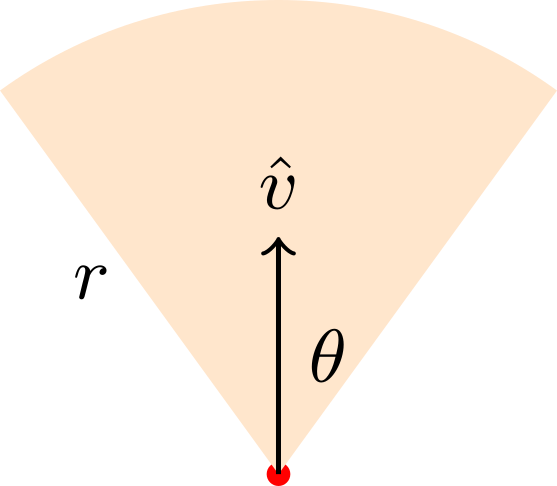
\includegraphics[width=0.3\linewidth]{immagini/fov.png}
  \caption{Rappresentazione del campo visivo di un pedone.}
  \label{fig:fov}
\end{figure}

% 2.1.3
\subsection{Movimento}
Lo spostamento dei pedoni all'interno di una folla, in maniera particolare durante un'evacuazione, non è dettato da una pianificazione del percorso da seguire ma da una serie di scelte attuate localmente analizzando le informazioni provenienti dall'ambiente circostante. Per modellare questi aspetti, mi sono avvalso dei comportamenti di steering formulati da C. W. Reynolds in \cite{Reynolds1999}, che sono alla base del movimento delle folle anche nel settore videoludico e in quello dell'animazione cinematografica. La loro funzione, infatti, è quella di muovere in maniera autonoma e realistica i personaggi su cui non si possiede il controllo, all'interno del mondo artificiale nel quale sono inseriti. \newline
Un comportamento di steering è una forza che influisce sul movimento di un agente al fine di permettergli di conseguire l'obiettivo per cui è pensato. Per determinarla ci si basa sulla semplice formula $steering = desired\_velocity - current\_velocity$, dove $current\_velocity$ è la direzione di movimento che l'agente sta seguendo, mentre $desired\_velocity$ è quella che egli vorrebbe seguire per adempiere il più velocemente possibile al suo intento. Nel caso il pedone non si stia muovendo, ovviamente, quest'ultima coinciderebbe con la forza di steering. \newline
Tra i comportamenti presenti si è focalizzata l'attenzione su quelli considerati più idonei a poter essere utilizzati nell'ambito dell'evacuazione di folle.

\paragraph{Raggiungere o fuggire}
I comportamenti più semplici a cui si può pensare nell'ambito dello steering sono il raggiungimento di un determinato punto di interesse all'interno dell'ambiente e, analogamente, la fuga da un luogo specificato, ad esempio per la presenza di un potenziale pericolo in corrispondenza ad esso.
Queste due forze, sono logicamente una l'opposto dell'altra, infatti, le $desired\_velocity$ relative ad ognuna di esse hanno direzioni contrarie.

\paragraph{Arrivare} 
Normalmente, quando un agente si trova in prossimità del punto che vuole raggiungere, esso è portato naturalmente a rallentare la propria velocità di andatura in maniera tale da arrivare a fermarsi in prossimità esatta del punto in questione. Questo risultato può essere ottenuto a partire dal già citato comportamento del raggiungimento, creando un cerchio intorno alla posizione d'interesse, detto \text{area di rallentamento} e scalando la velocità del pedone, nel caso vi si trovi all'interno di un fattore pari a $\frac{dist(p)}{radius}$, dove $dist(p)$ è la distanza corrente tra l'agente e il punto $p$ mentre $radius$ è il raggio dell'area di rallentamento.

\paragraph{Girovagare}
Volendo muovere un agente in maniera casuale si potrebbe pensare, riutilizzando concetti già analizzati, di generare periodicamente delle posizioni d'interesse fittizie all'interno dell'ambiente e di usufruire del comportamento \enquote{raggiungere} per indurre il pedone ad avvicinarvisi. Questo approccio però, potrebbe portare a movimenti innaturali dovuti a repentini cambi di direzione. \newline
Per ovviare a questo problema viene creata un circonferenza davanti dell'agente, sulla quale viene scelto casualmente un punto che sarà quello da raggiungere. Questa soluzione restringe il campo delle possibili posizioni verso cui dirigersi e determina risultati più simili al reale comportamento umano.

\paragraph{Evitare gli ostacoli} 
Considerando la potenziale presenza di ostacoli nell'ambiente, è necessario definire un comportamento di steering che permetta di schivarli in modo da evitare situazioni nelle quali un agente, a seguito di una collisione, rimanga per sempre bloccato, incapace di proseguire per via della presenza dell'ostacolo ma volendo al contempo andare al di là di esso. \newline
Ricordando che un agente ha una conoscenza limitata dell'ambiente circostante, in quanto le sue scelte sono localizzate, non viene presa in considerazione la totalità degli ostacoli presenti ma solo quello attualmente più prossimo ad esso. \newline
Per determinare il cambiamento di direzione, si usa la futura posizione di collisione e si applica una forza di repulsione considerando dove si trova il centro dell'ostacolo di riferimento. Tale formulazione, è particolarmente adatta per ostacoli di forma circolare, ma è utilizzabile potenzialmente per ogni tipo di ostacolo, approssimandone la forma a quella di un cerchio.

\paragraph{Seguire il flusso}
Il movimento di un agente potrebbe anche non essere guidato da una decisione ma da un fattore esterno in grado, direttamente o indirettamente, di determinare la prossima posizione in cui esso si troverà. Classici esempi sono le correnti d'acqua, in grado di trascinare, nel loro caotico movimento, gli eventuali oggetti che si trovano sulla loro strada, ma anche il campo magnetico, che, pur se non macroscopicamente osservabile, ha effetti evidenti in presenza di materiali ferrosi. \newline
Generalizzando questo fenomeno, è possibile modellarlo come un campo vettoriale, in cui ad ogni posizione è associata la prossima direzione da seguire che rappresenta appunto la $desired\_velocity$ di questo comportamento.

\subsubsection{Composizione di forze}
Pur potendo essere sfruttate anche singolarmente, le vere potenzialità dei comportamenti di steering possono essere apprezzate solo combinando i vari apporti tra loro in modo da ricreare dei movimenti complessi. In una situazione realistica, infatti, un pedone è in grado di decidere la prossima direzione da seguire, valutando contemporaneamente quella che gli consente di evitare gli ostacoli presenti, fuggire da situazioni di pericolo e raggiungere il prima possibile il punto di interesse. \newline
Questa tendenza è presente anche nella formulazione del modello forze sociali in tutte le sue varianti \cite{Chen2017}, dove, per ogni aspetto considerato, viene calcolata una forza che lo possa rappresentare realisticamente e tra queste viene poi eseguita la somma vettoriale per determinare la direzione e la velocità con cui il pedone deciderà di muoversi.

% 2.1.4
\subsection{Gruppi}
Considerare una folla come un aggregato di persone isolate è una semplificazione non sempre accettabile visto che più del 70\% dei pedoni si muove in gruppi \cite{Moussad2010}, che siano questi coppie, famiglie o amici. \newline
L'influenza del gruppo sul singolo individuo ad esso appartenente, è fondamentale per riprodurre dei comportamenti comuni nella vita di tutti i giorni, come la tendenza a rimanere uniti e a muoversi all'unisono aspettando coloro che sono eventualmente rimasti indietro. L'appartenenza ad un gruppo, infatti, non definisce solamente uno stato sociale per il pedone ma influisce in maniera decisiva anche sul suo movimento.

\subsubsection{Movimento collettivo}
In aggiunta ai comportamenti di steering precedentemente trattati, è possibile classificare altri atteggiamenti che scaturiscono nel pedone dalla necessità ad adattarsi al movimento degli altri individui presenti, in particolare se essi appartengono al suo stesso gruppo. \newline
Questa tendenza a conformarsi è visibile anche nel mondo naturale, dove lo spostamento in massa è una caratteristica peculiare di molte specie quali uccelli, pesci, batteri e insetti; è proprio dall'osservazione del loro comportamento che C. W. Reynolds ha formulato in \cite{Reynolds1987} le azioni alla base del movimento collettivo. \newline
Questi comportamenti, pur coinvolgendo più pedoni, sono a tutti gli effetti delle forze di steering e, in quanto tali, possono essere combinati tra loro per descrivere aspetti più complessi. Rispetto a quelli precedentemente descritti però, hanno un ruolo molto diverso. Infatti, mentre gli altri analizzano il movimento in relazione all'ambiente e non alla conformazione della folla presente, che potrebbe essere costituita anche da un solo pedone, le azioni collettive non avrebbero alcun effetto senza includere quest'ultimo aspetto. \newline
Per questo motivo, considerando l'introduzione dei gruppi nel modello forze sociali studiato in \cite{Moussad2010}, la direzione da seguire è stata calcolata considerando come contributi separati l'apporto delle semplici azioni di steering e di quelle di gruppo, piuttosto che mischiando insieme i comportamenti delle due categorie.

\paragraph{Allineamento}
La direzione e la velocità dei soggetti intorno ad un determinato pedone, determina su di esso una tendenza a conformarsi a questi parametri e a regolarli in modo da seguire il loro stesso andamento. Per riuscire in questo intento, il calcolo della direzione e del modulo della $desired\_velocity$ di questo comportamento in un pedone, viene effettuato considerando la media di questi fattori, negli individui entro una distanza massima predefinita da esso.

\paragraph{Coesione}
Analogamente a quanto definito nell'allineamento per velocità e direzione, un pedone è portato anche a spostarsi in posizioni che gli permettano di mantenere una certa vicinanza con gli altri individui presenti. Per calcolare il movimento che favorisca questo principio, si utilizza il centroide, cioè il punto medio delle posizioni attuali dei pedoni presi in considerazione. \newline
L'effetto del meccanismo di coesione tra i vari pedoni, ha ancor più rilevanza se considerato per gruppi già definiti \cite{Vizzari2013}, dove quella di rimanere uniti è la priorità anche rispetto a mettersi in salvo.

\paragraph{Separazione}
In maniera opposta al comportamento di coesione, se la densità di persone inizia a diventare proibitiva nelle immediate vicinanze di un pedone e vi è dello spazio disponibile da occupare, l'agente tenterà di andarci, in modo da ristabilire una certa distanza dagli altri e ottimizzare lo spazio che l'ambiente mette a disposizione.

\subsubsection{La presenza di leader}
Vi sono dei casi in cui i soggetti appartenenti ad un gruppo non hanno tutti la stessa rilevanza nella scelta del processo decisionale da attuare; ne è un esempio significativo quello della famiglia, in cui i figli tendono a seguire le indicazioni dei genitori, figure più consce della situazione che si è venuta a creare e con più esperienza su come risolverla. \newline
La presenza all'interno del gruppo di un leader, è un fattore determinante nello studio dell'evacuazione di folle \cite{Ji2006}\cite{Kster2011}, che agisce sensibilmente sulle scelte comportamentali degli altri membri, naturalmente portati dalla fiducia per esso, a seguire le sue indicazioni senza preoccuparsi delle eventuali conseguenze.